\documentclass[a4paper,10pt]{article}
\usepackage[left=1.5cm, right=1.5cm, top=2cm, bottom=2cm]{geometry}
\usepackage{graphicx}
\usepackage{booktabs}
\usepackage{caption}
\usepackage{subcaption}
\usepackage{listings} % For code formatting
\usepackage{xcolor} % For better code formatting
\usepackage{placeins} % fix page break issue
\usepackage{float}
\lstset{
    basicstyle=\ttfamily\small,
    breaklines=true,
    frame=single,
    xleftmargin=5pt,
    xrightmargin=5pt,
    backgroundcolor=\color{lightgray},
    keywordstyle=\color{blue},
    commentstyle=\color{green},
    stringstyle=\color{red}
}

\title{Assignment 1 - Visual Gallery based on MIMIC data using python libraries}
\author{Roofi Shaikh }
\date{\today}

\begin{document}

\maketitle

\section{Story 1: Insurance Type Distribution Over Years}

\subsection{Overview}
This analysis presents the distribution of patient insurance types over the years using MIMIC-III data. The visualization provides an overview of how different insurance types are represented across all recorded years.

\subsection{BigQuery Logic}
The following BigQuery query extracts patient admission records, groups them by insurance type and year, and pivots the data to create a structured view of insurance type distributions over time.

\begin{lstlisting}[language=SQL]
%%bigquery df --project bigaquery-aihc-assign1
SELECT * 
FROM (
  SELECT EXTRACT(YEAR FROM admittime) AS year, insurance 
  FROM `physionet-data.mimiciii_clinical.admissions`
)
PIVOT (
  COUNT(*) FOR insurance IN ('Medicare', 'Medicaid', 'Private', 'Self Pay', 'Government')
)
ORDER BY year;
\end{lstlisting}

\subsection{Heatmap Analysis}

\subsubsection{Visualization Code}
\begin{lstlisting}[language=Python]
import pandas as pd
import seaborn as sns
import matplotlib.pyplot as plt

# Convert all columns to standard int64 (fixes Seaborn error)
df = df.astype(int)  

# Convert index (years) to standard int
df.index = df.index.astype(int)

# Set figure size
plt.figure(figsize=(12, 12))

# Convert all values to numeric (ignoring errors)
df = df.apply(pd.to_numeric, errors='coerce')

# Create the heatmap
sns.heatmap(df, cmap="coolwarm", annot=True, fmt="d", linewidths=0.5)

# Set title and labels
plt.title("Heatmap of Insurance Type Distribution Over Years")
plt.xlabel("Insurance Type")
plt.ylabel("Year")

# Save the plot
plt.savefig("figure1a.png")
\end{lstlisting}

\subsubsection{Visualization}

\begin{figure}[h]
    \centering
    \includegraphics[width=0.8\textwidth]{figure1a.png}
    \caption{Heatmap showing distribution of insurance types over the years.}
    \label{fig:heatmap}
\end{figure}

\subsubsection{Insights}
- Heatmap shows distribution of number of patients covered for each year by each insurance type.

\subsection{Bar Chart Analysis}

\subsubsection{Visualization Code}
\begin{lstlisting}[language=Python]
import pandas as pd
import matplotlib.pyplot as plt

# Sum patient counts for each insurance type across all years
insurance_totals = df.sum(axis=0)

# Set figure size
plt.figure(figsize=(10, 6))

# Create a bar chart
insurance_totals.plot(kind="bar", color=["blue", "orange", "green", "red", "purple"])

# Add labels and title
plt.title("Total Patients Covered by Each Insurance Type (All Years)")
plt.xlabel("Insurance Type")
plt.ylabel("Total Patients")
plt.xticks(rotation=45)

# Save the plot
plt.savefig("figure1b.png")
\end{lstlisting}

\subsubsection{Visualization}

\begin{figure}[h]
    \centering
    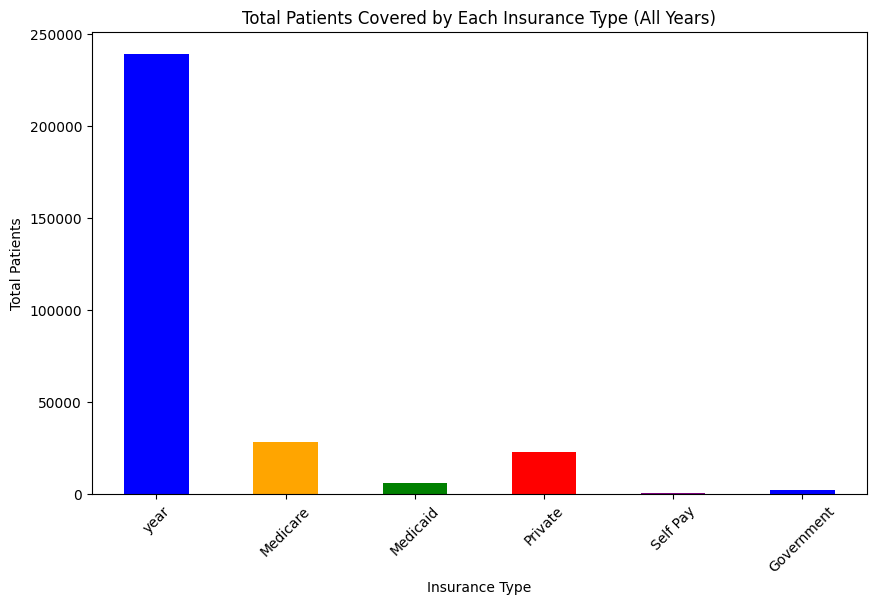
\includegraphics[width=0.8\textwidth]{figure1b.png}
    \caption{Bar chart of total patients covered by each insurance type.}
    \label{fig:bar_chart}
\end{figure}

\subsubsection{Insights}
- The bar chart shows the total number of patients covered by each insurance type.

\subsection{Pie Chart Analysis}

\subsubsection{Visualization Code}
\begin{lstlisting}[language=Python]
import pandas as pd
import matplotlib.pyplot as plt

# Display proportion of each insurance type across years
plt.figure(figsize=(8, 8))

# Create a pie chart
insurance_totals.plot(kind="pie", autopct="%1.1f%%", colors=["blue", "orange", "green", "red", "purple"])

# Add title
plt.title("Proportion of Patients Covered by Each Insurance Type (All Years)")

plt.ylabel("")  # Hide y-axis label

# Save the plot
plt.savefig("figure1c.png")
\end{lstlisting}

\subsubsection{Visualization}

\begin{figure}[h]
    \centering
    \includegraphics[width=0.8\textwidth]{figure1c.png}
    \caption{Pie chart showing the proportion of patients covered by each insurance type.}
    \label{fig:pie_chart}
\end{figure}

\subsubsection{Insights}
- The pie chart shows the proportion of patients covered by each insurance type across all recorded years.

%%%%% Section 2 for 2nd Story %%%%%
\section{The Weekend Effect – Are Patients Admitted on Weekends More Likely to Die?}

\subsection{Research Question}
Are patients admitted on weekends (Saturday \& Sunday) more likely to die in the hospital compared to weekday admissions? Do certain ICU types (Medical vs. Surgical) have higher mortality rates on weekends?

\subsection{BigQuery Logic}
The following BigQuery query analyzes hospital mortality rates based on admission day and ICU type.

\begin{lstlisting}[language=SQL]
%%bigquery df --project bigaquery-aihc-assign1
WITH AdmissionAnalysis AS (
  SELECT 
    a.subject_id,
    a.hadm_id,
    icu.first_careunit AS icu_type,
    a.hospital_expire_flag,
    EXTRACT(DAYOFWEEK FROM a.admittime) AS admit_day,
    CASE 
      WHEN EXTRACT(DAYOFWEEK FROM a.admittime) IN (1, 7) THEN 'Weekend'
      ELSE 'Weekday'
    END AS admission_type
  FROM `physionet-data.mimiciii_clinical.admissions` a
  LEFT JOIN `physionet-data.mimiciii_clinical.icustays` icu 
    ON a.hadm_id = icu.hadm_id
)
SELECT 
  admission_type,
  icu_type,
  COUNT(*) AS total_admissions,
  SUM(hospital_expire_flag) AS total_deaths,
  ROUND(SUM(hospital_expire_flag) / COUNT(*) * 100, 2) AS mortality_rate
FROM AdmissionAnalysis
GROUP BY admission_type, icu_type
ORDER BY admission_type, mortality_rate DESC;
\end{lstlisting}

\subsection{Visualization Logic}
The visualization represents the mortality rate of ICU patients admitted on weekends versus weekdays. The mortality rate is calculated for each ICU type and grouped by admission type (Weekday vs. Weekend). A bar chart is used to highlight the differences in mortality rates among different ICU types. The annotation on top of the bars provides precise mortality rate percentages for better clarity.

\subsection{Visualization Code}
\begin{lstlisting}[language=Python]
# Convert admission type to categorical for proper ordering
df["admission_type"] = pd.Categorical(df["admission_type"], categories=["Weekday", "Weekend"], ordered=True)

# Set figure size
plt.figure(figsize=(10, 6))

# Create the bar chart
ax = sns.barplot(x="icu_type", y="mortality_rate", hue="admission_type", data=df, palette="coolwarm")

# Add labels (percentage values) on top of each bar
for p in ax.patches:
    ax.annotate(f'{p.get_height():.1f}%', 
                (p.get_x() + p.get_width() / 2., p.get_height()), 
                ha='center', va='bottom', fontsize=12, fontweight='bold', color='black')

# Customize plot
plt.title("Mortality Rate by ICU Type (Weekday vs. Weekend)")
plt.xlabel("ICU Type")
plt.ylabel("Mortality Rate (%)")
plt.legend(title="Admission Type")

# Show the plot
plt.show()
\end{lstlisting}

\subsection{Visualization}

\subsubsection{Mortality Rate Bar Chart}
\begin{figure}[h]
    \centering
    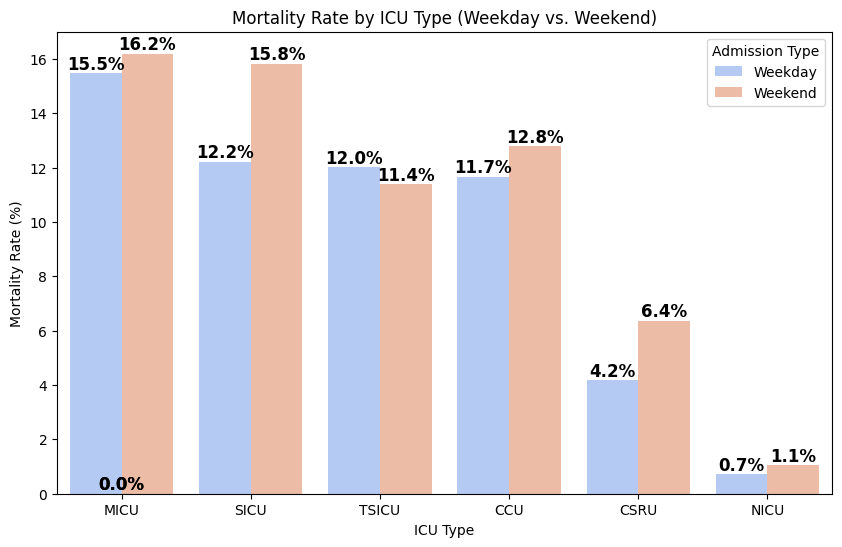
\includegraphics[width=0.8\textwidth]{figure2.png}
    \caption{Mortality Rate by ICU Type (Weekday vs. Weekend).}
    \label{fig:weekend_effect}
\end{figure}

\subsection{Insights}
- From the above graph, it indicates that the mortality rate is higher on weekends than weekdays for all ICU types except TSICU.

%%% Story 3 ----
\section{What Predicts a 30-Day Readmission?}

\subsection{Motivation for Analyzing 30-Day Hospital Readmissions}
Hospital readmissions within \textbf{30 days of discharge} are a critical healthcare challenge, leading to \textbf{increased costs, resource strain, and potential gaps in patient care}. Identifying the \textbf{most common reasons for readmission} allows hospitals to \textbf{proactively monitor high-risk conditions}, improve \textbf{discharge planning}, and implement \textbf{preventative strategies} to reduce avoidable returns.

Using \textbf{MIMIC-III}, a comprehensive ICU patient dataset, we analyze readmissions to uncover \textbf{the most frequent causes}. Instead of relying on assumptions, we let the \textbf{data reveal the top reasons} why patients return. By filtering out low-frequency occurrences, we ensure that our insights focus on \textbf{clinically significant trends} that hospitals can act upon.

The \textbf{TreeMap visualization} helps group similar diagnoses, providing a clear overview of major contributing factors. A \textbf{Heatmap} further illustrates trends over time, helping hospitals identify \textbf{seasonal or progressive risks}. These visualizations make complex data \textbf{intuitive and actionable}, aiding hospital administrators, clinicians, and policymakers in \textbf{targeted interventions}.

By focusing on \textbf{data-driven decision-making}, this analysis aims to \textbf{reduce unnecessary readmissions}, enhance \textbf{patient outcomes}, and optimize \textbf{hospital resource allocation}.

\subsection{BigQuery Logic}
The following BigQuery query extracts 30-day readmissions and identifies the most frequent diagnoses leading to readmission.

\begin{lstlisting}[language=SQL]
WITH readmissions AS (
    SELECT 
        hadm_id,
        subject_id,
        admittime,
        dischtime,
        LAG(dischtime) OVER (PARTITION BY subject_id ORDER BY admittime) AS prev_discharge,
        DATETIME_DIFF(admittime, LAG(dischtime) OVER (PARTITION BY subject_id ORDER BY admittime), DAY) AS days_since_discharge
    FROM `physionet-data.mimiciii_clinical.admissions`
),
filtered_readmissions AS (
    SELECT 
        r.hadm_id,
        r.subject_id,
        r.admittime,
        r.dischtime,
        r.days_since_discharge,
        d.icd9_code
    FROM readmissions r
    JOIN `physionet-data.mimiciii_clinical.diagnoses_icd` d 
        ON r.hadm_id = d.hadm_id
    WHERE r.days_since_discharge BETWEEN 1 AND 30 -- Only include readmissions within 30 days
),
all_diagnoses AS (
    SELECT 
        icd9_code,
        COUNT(*) AS readmission_count
    FROM filtered_readmissions
    GROUP BY icd9_code
    HAVING readmission_count >= 10 -- Exclude single-digit readmissions
    ORDER BY readmission_count DESC
)
SELECT 
    a.icd9_code,
    d.long_title AS diagnosis_description,
    a.readmission_count
FROM all_diagnoses a
JOIN `physionet-data.mimiciii_clinical.d_icd_diagnoses` d 
    ON a.icd9_code = d.icd9_code
ORDER BY a.readmission_count DESC;
\end{lstlisting}

\subsection{Visualization Logic}
The TreeMap groups similar diagnoses together, visually representing the most common causes of 30-day hospital readmissions. Larger rectangles indicate a higher frequency of readmission due to a specific diagnosis. This helps hospitals identify key areas for intervention.

\subsection{Visualization Code}
\begin{lstlisting}[language=Python]
# Create an interactive TreeMap
fig_treemap = px.treemap(
    df,
    path=["diagnosis_description"],  # Group by diagnosis
    values="readmission_count",  # Size based on readmission frequency
    title="TreeMap of 30-Day Readmission Causes",
    color="readmission_count",
    color_continuous_scale="Reds",
    hover_data={"readmission_count": True}  # Enable interactive hover information
)

# Increase font size for labels
fig_treemap.update_traces(
    textinfo="label+value",
    textfont_size=16,  # Adjust this value to make labels bigger
    hoverinfo="label+value+percent entry"  # Enhance hover details
)

# Adjust layout for better visibility
fig_treemap.update_layout(
    margin=dict(l=10, r=10, t=50, b=10),
    title_font=dict(size=20)  # Increase title font size
)

# Show the interactive plot
fig_treemap.show()
\end{lstlisting}

\subsection{Visualization}
\begin{figure}[h]
    \centering
    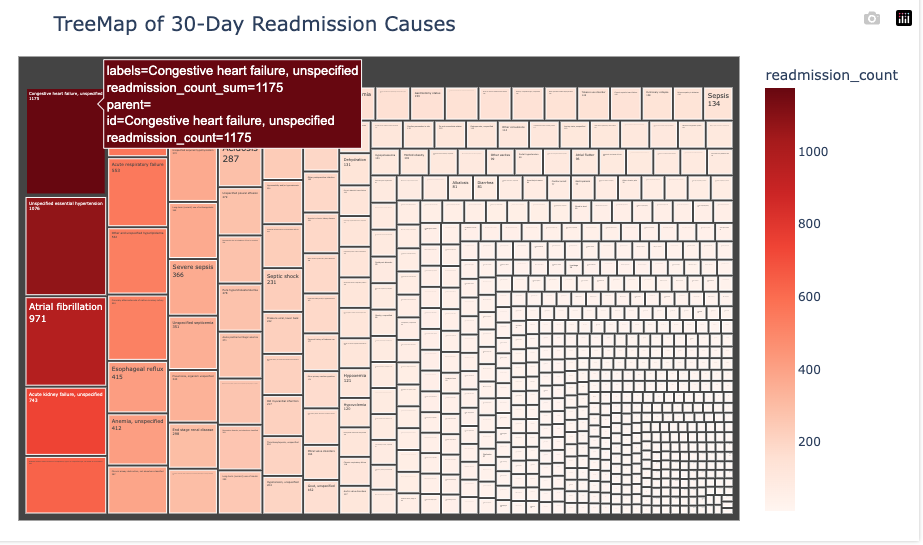
\includegraphics[width=0.8\textwidth]{figure3.png}
    \caption{Interactive TreeMap of 30-Day Readmission Causes.}
    \label{fig:readmission_treemap}
\end{figure}

\subsection{Insights}
The TreeMap provides a visual representation of the top ICD-9 causes of hospital readmission. Larger and darker rectangles indicate higher readmission rates, making it easy to identify the most frequent and critical conditions. This visualization helps hospitals focus on high-risk diagnoses, enabling better monitoring, targeted interventions, and improved patient care to reduce unnecessary readmissions.


%%%%% 
%%% Story 4 : Sepsis Mortality rates 
\section{Can Early Lactate and Creatinine Levels Predict Mortality in ICU Sepsis Patients?}

\subsection{Hypothesis}
High Lactate levels (>4 mmol/L) increase mortality risk. Creatinine may indicate kidney dysfunction but is a weaker predictor. Early detection of high-risk patients can improve ICU interventions.

\subsection{BigQuery Logic}
The following BigQuery query extracts sepsis patients and analyzes early Lactate and Creatinine levels within the first 6 hours of ICU admission.

\begin{lstlisting}[language=SQL]
-- Step 1: Identify Sepsis Patients
WITH sepsis_patients AS (
    SELECT 
        icu.subject_id, 
        icu.hadm_id, 
        icu.icustay_id,
        pat.gender,
        pat.dob AS birthdate,
        icu.intime AS icu_admit_time,
        icu.outtime AS icu_discharge_time,
        adm.hospital_expire_flag AS mortality -- 1 if patient died in hospital
    FROM `physionet-data.mimiciii_clinical.icustays` icu
    JOIN `physionet-data.mimiciii_clinical.admissions` adm 
        ON icu.hadm_id = adm.hadm_id
    JOIN `physionet-data.mimiciii_clinical.patients` pat
        ON icu.subject_id = pat.subject_id
)

-- Step 2: Lookup Item IDs for Key Lab Tests (Lactate, WBC, Creatinine)
, lab_items AS (
    SELECT itemid, label
    FROM `physionet-data.mimiciii_clinical.d_labitems`
    WHERE LOWER(label) IN ('lactate', 'white blood cell count', 'creatinine')
)

-- Step 3: Extract First Lab Measurement Within 6 Hours of ICU Admission
, early_lab_values AS (
    SELECT 
        le.subject_id, 
        le.hadm_id, 
        le.itemid, 
        le.charttime,
        le.valuenum AS lab_value,
        li.label AS lab_name
    FROM `physionet-data.mimiciii_clinical.labevents` le
    JOIN lab_items li 
        ON le.itemid = li.itemid
    JOIN sepsis_patients sp
        ON le.subject_id = sp.subject_id 
        AND le.hadm_id = sp.hadm_id
        AND le.charttime BETWEEN sp.icu_admit_time AND TIMESTAMP_ADD(sp.icu_admit_time, INTERVAL 6 HOUR)
)

-- Step 4: Combine Data Into Final Output
SELECT 
    s.subject_id, 
    s.hadm_id, 
    s.icustay_id, 
    s.gender,
    DATE_DIFF(CURRENT_DATE(), DATE(s.birthdate), YEAR) AS age,
    e.lab_name, 
    e.lab_value,
    s.mortality
FROM sepsis_patients s
LEFT JOIN early_lab_values e
ON s.subject_id = e.subject_id AND s.hadm_id = e.hadm_id
ORDER BY s.subject_id, s.hadm_id, e.charttime;
\end{lstlisting}

\subsection{Visualization Code}
\begin{lstlisting}[language=Python]
# Ensure mortality is numeric (0 = survived, 1 = died)
df['mortality'] = df['mortality'].astype(int)

sns.set(style="whitegrid")

### PLOT 1: Distribution of Key Lab Markers ###
plt.figure(figsize=(10, 5))

# Improved histogram with proper layering
sns.histplot(df, x="lab_value", hue="lab_name", bins=30, kde=True, multiple="layer", alpha=0.6)

# Properly position the legend
plt.legend(title="Lab Test", loc="upper right", fontsize=10)

# Titles and labels
plt.title("Distribution of Key Lab Markers in ICU Sepsis Patients", fontsize=14)
plt.xlabel("Lab Value", fontsize=12)
plt.ylabel("Count", fontsize=12)

plt.show()
\end{lstlisting}

\subsection{Visualization}

\begin{figure}[h]
    \centering
    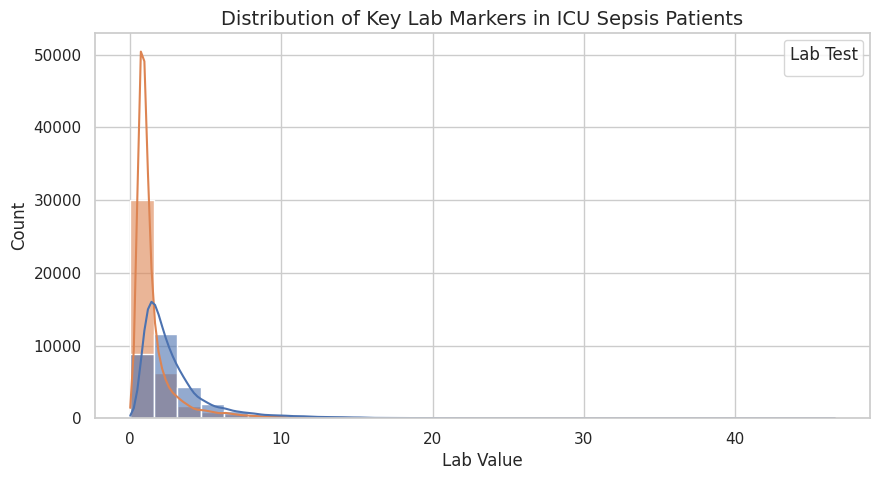
\includegraphics[width=0.8\textwidth]{figure4a.png}
    \caption{Distribution of Key Lab Markers in ICU Sepsis Patients.}
    \label{fig:lab_distribution}
\end{figure}

\begin{figure}[H]
    \centering
    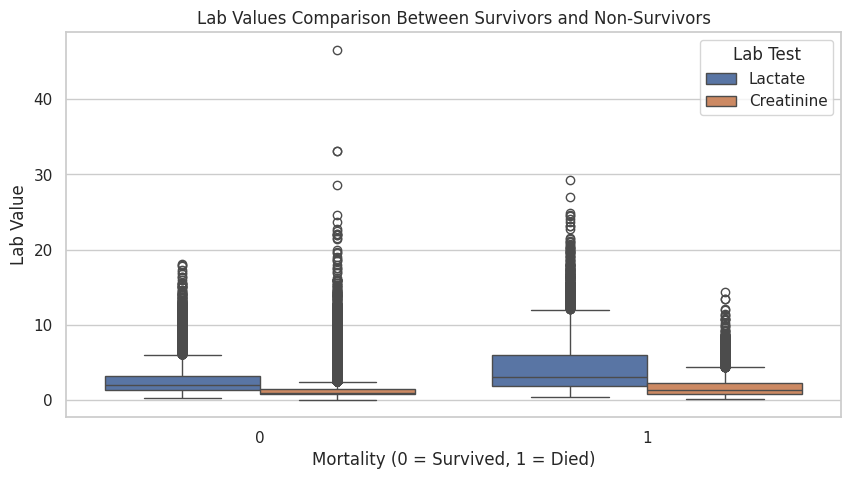
\includegraphics[width=0.8\textwidth]{figure4b.png}
    \caption{Lab values comparison between survivors and non-survivors.}
    \label{fig:lab_comparison}
\end{figure}

\begin{figure}[h]
    \centering
    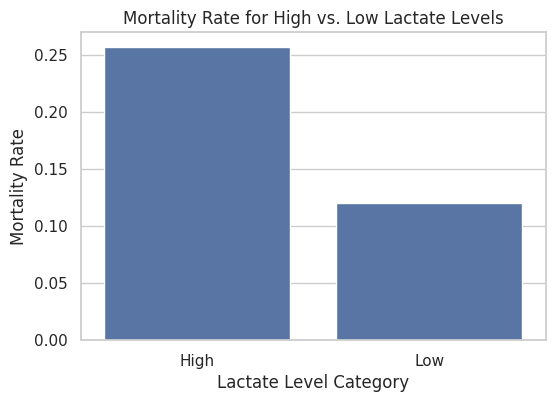
\includegraphics[width=0.8\textwidth]{figure4c.png}
    \caption{Mortality rate for high vs low lactate levels.}
    \label{fig:lactate_mortality}
\end{figure}

\begin{figure}[h]
    \centering
    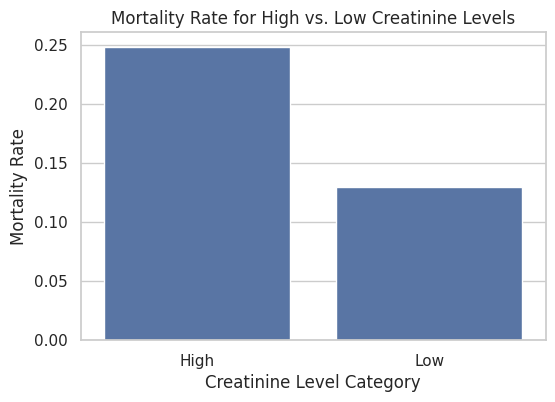
\includegraphics[width=0.8\textwidth]{figure4d.png}
    \caption{Mortality rate for high vs low creatinine levels.}
    \label{fig:creatinine_mortality}
\end{figure}

\clearpage

\subsection{Insights}
- High Lactate levels (\textgreater 4 mmol/L) are strongly correlated with increased mortality in ICU sepsis patients.
- Creatinine levels provide some indication of mortality risk but are a weaker predictor compared to Lactate.
- The boxplot shows a clear distinction in lab values between survivors and non-survivors, reinforcing the importance of early monitoring.
- Early detection of high-risk patients based on these biomarkers can lead to improved ICU interventions and patient outcomes.

%% Opiod Usage Story Section 


\section{Opioid Usage Across ICUs and Its Relationship to Hospital Stays}

\subsection{Study Overview}
This study analyzes opioid dosing patterns in ICU patients, exploring dosage distributions, prescription trends, and their impact on hospital stays. We investigate whether opioid usage follows standardized dosing protocols, identify variations across ICU types, and examine the relationship between opioid dosage and hospital length of stay. By comparing opioid prescription rates across different ICUs, we aim to uncover patterns in pain management strategies and assess whether higher opioid doses correlate with prolonged ICU stays. Understanding these trends can optimize opioid prescribing practices, reduce overuse risks, and enhance patient outcomes in critical care settings.

\subsection{BigQuery Logic}
The following BigQuery query extracts opioid usage data and assesses its impact on ICU length of stay.

\begin{lstlisting}[language=SQL]
WITH opioid_list AS (
    -- Dynamically fetch all opioid medication item IDs
    SELECT itemid 
    FROM `physionet-data.mimiciii_clinical.d_items`
    WHERE LOWER(label) LIKE '%fentanyl%'
        OR LOWER(label) LIKE '%morphine%'
        OR LOWER(label) LIKE '%oxycodone%'
        OR LOWER(label) LIKE '%hydromorphone%'
        OR LOWER(label) LIKE '%methadone%'
        OR LOWER(label) LIKE '%opioid%' -- Covers general opioid-related terms
),

opioid_data AS (
    SELECT 
        ie.icustay_id,
        ie.subject_id,
        ie.hadm_id,
        ie.starttime,
        ie.amount AS opioid_dosage, -- Opioid dosage administered
        icu.first_careunit AS icu_type, -- ICU type (Medical, Surgical, etc.)
        adm.admittime,
        adm.dischtime,
        DATE_DIFF(adm.dischtime, adm.admittime, DAY) AS hospital_length_of_stay
    FROM `physionet-data.mimiciii_clinical.inputevents_mv` ie
    JOIN `physionet-data.mimiciii_clinical.icustays` icu 
        ON ie.icustay_id = icu.icustay_id
    JOIN `physionet-data.mimiciii_clinical.admissions` adm 
        ON ie.hadm_id = adm.hadm_id
    JOIN opioid_list ol 
        ON ie.itemid = ol.itemid -- Dynamically filter opioid medications
)

SELECT 
    icustay_id,
    subject_id,
    opioid_dosage,
    hospital_length_of_stay,
    icu_type
FROM opioid_data;
\end{lstlisting}

\subsection{Visualization Code}
\begin{lstlisting}[language=Python]
# Function to clean and visualize opioid usage data
def visualize_opioid_usage_fixed(df):
    """
    Generates three visualizations with improved data filtering:
    1. Histogram of opioid dosages (filtered)
    2. Scatter plot of opioid dosage vs. hospital length of stay (filtered)
    3. Bar chart of opioid prescription rate by ICU type
    """

    # 1. Fix Histogram - Opioid Dosage Distribution
    df_filtered = df[df["opioid_dosage"] > 0]  # Remove negative values
    upper_limit = np.percentile(df_filtered["opioid_dosage"], 99)  # Find the 99th percentile
    df_filtered = df_filtered[df_filtered["opioid_dosage"] <= upper_limit]  # Remove extreme outliers

    plt.figure(figsize=(8, 5))
    sns.histplot(df_filtered["opioid_dosage"], bins=30, kde=True, color="blue")
    plt.title("Distribution of Opioid Dosages in ICU Patients (Filtered)")
    plt.xlabel("Opioid Dosage (mg)")
    plt.ylabel("Number of Patients")
    plt.show()
\end{lstlisting}

\clearpage % Forces the section to start on a new page

\subsection{Visualization}

\begin{figure}[h]
    \centering
    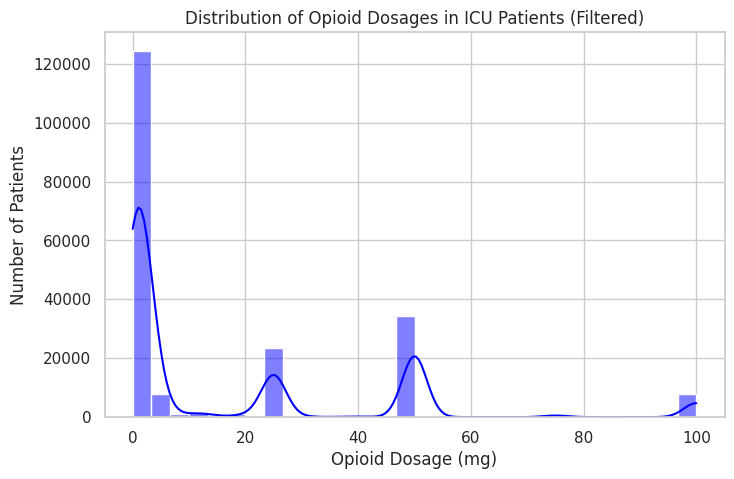
\includegraphics[width=0.8\textwidth]{figure5a.png}
    \caption{Distribution of Opioid Dosages in ICU Patients.}
    \label{fig:opioid_distribution}
\end{figure}

\begin{figure}[H]
    \centering
    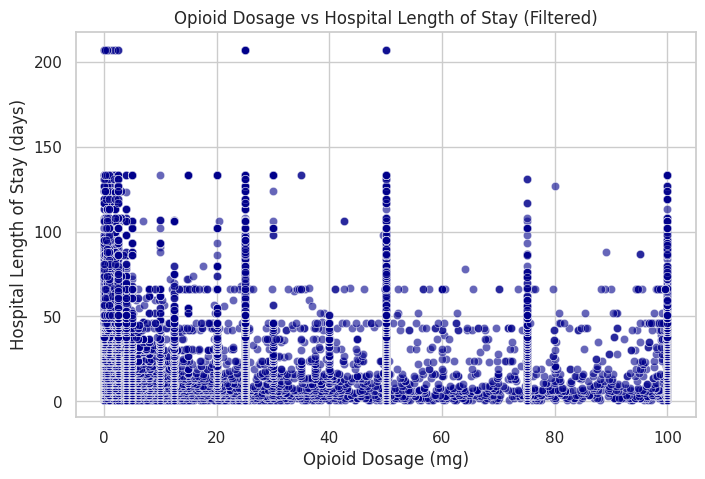
\includegraphics[width=0.8\textwidth]{figure5b.png}
    \caption{Opioid Dosage vs Hospital Length of Stay.}
    \label{fig:opioid_vs_stay}
\end{figure}

\begin{figure}[H]
    \centering
    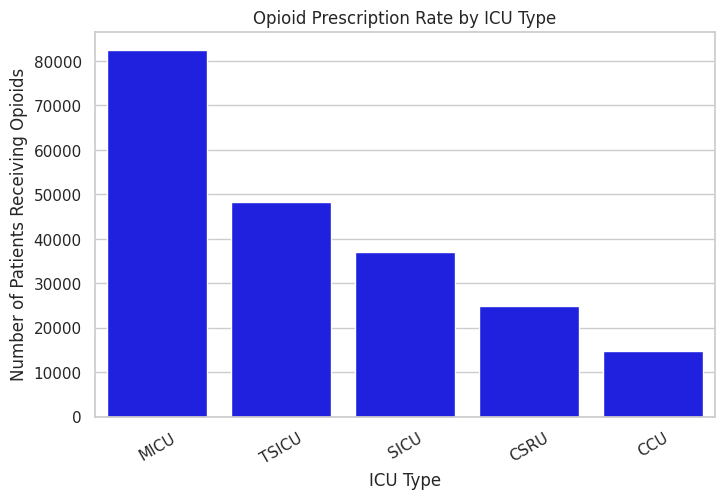
\includegraphics[width=0.8\textwidth]{figure5c.png}
    \caption{Opioid Prescription Rate by ICU Type.}
    \label{fig:opioid_prescription_rate}
\end{figure}



\subsection{Insights}
- The histogram shows that most ICU patients receive no opioids, while some receive standard dosages around 20 mg, 40 mg, and a few reaching 90 mg.
- The scatter plot does not reveal a clear relationship between opioid dosage and hospital length of stay, indicating that other factors may influence duration.
- The bar chart indicates that opioid prescription rates are highest in MICU, followed by TSICU, SICU, CSRU, and CCU, showing variation in pain management across ICU types.
\clearpage

\end{document}
